\documentclass[12pt,a4paper]{article}

\usepackage{geometry}
\geometry{total={210mm,297mm},
left=20mm,right=20mm,top=20mm,bottom=20mm}

\usepackage[utf8]{inputenc}
\usepackage[T1]{fontenc}
\usepackage{graphicx}
\usepackage{amsmath,amssymb}
\usepackage{xcolor}
\usepackage{siunitx}
\usepackage{lineno}
\usepackage{cite}
\usepackage{stfloats}
\usepackage{subcaption}
\usepackage{avant}
\usepackage{hyperref}
\hypersetup{
  colorlinks,
  citecolor=black,
  filecolor=black,
  linkcolor=blue,
  urlcolor=black
}
\renewcommand\familydefault{\sfdefault}
\hypersetup{linktocpage}

\usepackage{longtable}

%\usepackage[french]{babel}
\usepackage[english]{babel}
\usepackage[T1]{fontenc}
\usepackage{fancyhdr}
\pagestyle{fancy}

\newcommand{\T}[1]{\boldsymbol{#1}}
\newcommand{\TT}[1]{\boldsymbol{#1}}
\newcommand{\TTTT}[1]{\underline{\boldsymbol{#1}}}

\usepackage[square,sort&compress,comma,numbers]{natbib}
%%%%%%%%%%%%%%%%%%%%%%%%%%%%%%%%%%%%%%%%%%%%%%%%%%
%%%%%%%%%%%%%%%%%%%%%%%%%%%%%%%%%%%%%%%%%%%%%%%%%%
%%%%%%%%%%%%%%%%%%%%%%%%%%%%%%%%%%%%%%%%%%%%%%%%%%

%%% Other Packages

\newcommand{\tenstwo}[1]{\boldsymbol{#1}}
\newcommand{\FF}{\tenstwo{F}}
\newcommand{\dotFF}{\dot{\tenstwo{F}}}
\newcommand{\detFF}{\mathrm{det}\FF}
\newcommand{\invFF}{\tenstwo{F}^{-1}}
\newcommand{\II}{\tenstwo{I}}
\newcommand{\LL}{\tenstwo{L}}
\newcommand{\vct}[1]{\boldsymbol{#1}}
\newcommand{\norm}[1]{\left\lVert#1\right\rVert}
\newcommand{\average}[1]{\left<#1\right>}

%\usepackage{kpfonts}
\usepackage{listings}
\usepackage{pgfplots}
%\usepackage{sansmath}
\usepackage{xcolor}

\usepackage{tikz}
%\usetikzlibrary{3d}
%\RequirePackage{3dplot}
\usetikzlibrary{calc}
\usetikzlibrary{arrows,positioning,shapes.geometric}
\usetikzlibrary{shapes.misc}

\tikzset{cross/.style={cross out, draw,
    minimum size=2*(#1-\pgflinewidth),
             inner sep=0pt, outer sep=0pt}, cross/.default={1pt}}

\pgfplotsset{compat=newest}
\usepgfplotslibrary{groupplots} 
%\RequirePackage{tikz-uml}
\RequirePackage{listings}

\definecolor{step1gsf}{RGB}{31,0,0}
\definecolor{step2gsf}{RGB}{131,0,0}
\definecolor{step3gsf}{RGB}{255,138,5}
\definecolor{step4gsf}{RGB}{227,41,0}
\definecolor{step5gsf}{RGB}{255,216,21}

\definecolor{viridis1}{HTML}{440154}
\definecolor{viridis2}{HTML}{481567}
\definecolor{viridis3}{HTML}{482677}
\definecolor{viridis4}{HTML}{453781}
\definecolor{viridis5}{HTML}{404788}
\definecolor{viridis6}{HTML}{39568C}
\definecolor{viridis7}{HTML}{33638D}
\definecolor{viridis8}{HTML}{2D708D}
\definecolor{viridis9}{HTML}{287D8E}
\definecolor{viridis10}{HTML}{238A8D}
\definecolor{viridis11}{HTML}{1F968B}
\definecolor{viridis12}{HTML}{20A387}
\definecolor{viridis13}{HTML}{29AF7F}
\definecolor{viridis14}{HTML}{3CBB75}
\definecolor{viridis15}{HTML}{55C667}
\definecolor{viridis16}{HTML}{73D055}
\definecolor{viridis17}{HTML}{95D840}
\definecolor{viridis18}{HTML}{B8DE29}
\definecolor{viridis19}{HTML}{DCE319}
\definecolor{viridis20}{HTML}{FDE725}


%%% cea
\definecolor{redCEA}{RGB}{220,5,40}
\definecolor{greyCEA}{RGB}{102,102,102}
\definecolor{greenCEA}{RGB}{15,113,39}

\definecolor{redCEA_light}{RGB}{230,0,25}
\definecolor{greenCEA_light}{RGB}{145,195,10}
\definecolor{greyCEA_light}{RGB}{227,227,227}

\definecolor{bleuP}{rgb}{0.02, 0.38, 0.67}
\definecolor{vertI}{rgb}{0.0, 0.90, 0.50}
\definecolor{redF}{rgb}{0.81, 0.00, 0.00}


%%% nice red
\definecolor{myRed}{RGB}{157,16,45}

\definecolor{grad1}{RGB}{15,113,39}
\definecolor{grad2}{RGB}{43,134,14}
\definecolor{grad3}{RGB}{115,155,13}
\definecolor{grad4}{RGB}{177,144,11}
\definecolor{grad5}{RGB}{198,69,8}
\definecolor{grad6}{RGB}{220,5,40}


%%% ensta paristech
\definecolor{blueEnsta}{RGB}{1,132,184} 


%%% los alamos laboratory
\definecolor{blueLanl}{RGB}{62,16,124}


%%% Some colors

\definecolor{linebnearlytransparent}{RGB}{212,228,242}

\definecolor{line01}{RGB}{242, 201,  49}
\definecolor{line02}{RGB}{ 33, 110, 180}
\definecolor{line03}{RGB}{154, 153,  64}
\definecolor{line04}{RGB}{187,  77, 152}
\definecolor{line05}{RGB}{222, 139,  83}
\definecolor{line06}{RGB}{121, 187, 146}
\definecolor{line07}{RGB}{223, 154, 177}
\definecolor{line08}{RGB}{197, 163, 202}
\definecolor{line09}{RGB}{205, 200,  63}
\definecolor{line10}{RGB}{223, 176,  57}
\definecolor{line11}{RGB}{142, 101,  56}
\definecolor{line12}{RGB}{ 50, 142,  91}
\definecolor{line13}{RGB}{137, 199, 214}
\definecolor{line14}{RGB}{103,  50, 142}

\definecolor{linea}{RGB}{211,  94,  60}
\definecolor{lineb}{RGB}{ 78, 144, 204}
\definecolor{linec}{RGB}{232, 203,  14}
\definecolor{lined}{RGB}{ 23, 150,  76}
\definecolor{linee}{RGB}{199,  95, 173}

%%% Graph Colors

\colorlet{clr_def}{lineb!33}
\colorlet{clr_sse}{lineb!67}
\colorlet{clr_avx}{lineb}

\colorlet{clr_mpi}{lineb!33}
\colorlet{clr_h_2}{lineb!67}
\colorlet{clr_h_4}{lineb}
\colorlet{clr_tbb}{line05!80}

\colorlet{clr_background}{lineb!25}
\colorlet{clr_edge}{line02}
\colorlet{clr_struct}{line05}
\colorlet{clr_text}{red}

\colorlet{clr_1_th}{line01}
\colorlet{clr_2_th}{lineb}
\colorlet{clr_4_th}{line06}
\colorlet{clr_8_th}{line05}
\colorlet{clr_16_th}{linea}

\definecolor{indigo}{RGB}{75 0 130}
\definecolor{gold}{RGB}{255 215 0}
\definecolor{hotpink}{RGB}{255 105 180}
\definecolor{firebrick}{RGB}{178 34 34}
\definecolor{indianred}{RGB}{205 92 92}
\definecolor{yellow}{RGB}{255 255 0}
\definecolor{mistyrose}{RGB}{255 228 225}
\definecolor{darkolivegreen}{RGB}{85 107 47}
\definecolor{olive}{RGB}{128 128 0}
\definecolor{darkseagreen}{RGB}{143 188 143}
\definecolor{pink}{RGB}{255 192 203}
\definecolor{lightcoral}{RGB}{240 128 128}
\definecolor{orangered}{RGB}{255 69 0}
\definecolor{navajowhite}{RGB}{255 222 173}
\definecolor{lime}{RGB}{0 255 0}
\definecolor{palegreen}{RGB}{152 251 152}
\definecolor{darkslategrey}{RGB}{47 79 79}
\definecolor{greenyellow}{RGB}{173 255 47}
\definecolor{burlywood}{RGB}{222 184 135}
\definecolor{seashell}{RGB}{255 245 238}
\definecolor{mediumspringgreen}{RGB}{0 250 154}
\definecolor{fuchsia}{RGB}{255 0 255}
\definecolor{papayawhip}{RGB}{255 239 213}
\definecolor{blanchedalmond}{RGB}{255 235 205}
\definecolor{chartreuse}{RGB}{127 255 0}
\definecolor{dimgray}{RGB}{105 105 105}
\definecolor{black}{RGB}{0 0 0}
\definecolor{peachpuff}{RGB}{255 218 185}
\definecolor{springgreen}{RGB}{0 255 127}
\definecolor{aquamarine}{RGB}{127 255 212}
\definecolor{white}{RGB}{255 255 255}
\definecolor{orange}{RGB}{255 165 0}
\definecolor{lightsalmon}{RGB}{255 160 122}
\definecolor{darkslategray}{RGB}{47 79 79}
\definecolor{brown}{RGB}{165 42 42}
\definecolor{ivory}{RGB}{255 255 240}
\definecolor{dodgerblue}{RGB}{30 144 255}
\definecolor{peru}{RGB}{205 133 63}
\definecolor{darkgrey}{RGB}{169 169 169}
\definecolor{lawngreen}{RGB}{124 252 0}
\definecolor{chocolate}{RGB}{210 105 30}
\definecolor{crimson}{RGB}{220 20 60}
\definecolor{forestgreen}{RGB}{34 139 34}
\definecolor{slateblue}{RGB}{106 90 205}
\definecolor{lightseagreen}{RGB}{32 178 170}
\definecolor{cyan}{RGB}{0 255 255}
\definecolor{mintcream}{RGB}{245 255 250}
\definecolor{silver}{RGB}{192 192 192}
\definecolor{antiquewhite}{RGB}{250 235 215}
\definecolor{mediumorchid}{RGB}{186 85 211}
\definecolor{skyblue}{RGB}{135 206 235}
\definecolor{gray}{RGB}{128 128 128}
\definecolor{darkturquoise}{RGB}{0 206 209}
\definecolor{goldenrod}{RGB}{218 165 32}
\definecolor{darkgreen}{RGB}{0 100 0}
\definecolor{floralwhite}{RGB}{255 250 240}
\definecolor{darkviolet}{RGB}{148 0 211}
\definecolor{darkgray}{RGB}{169 169 169}
\definecolor{moccasin}{RGB}{255 228 181}
\definecolor{saddlebrown}{RGB}{139 69 19}
\definecolor{grey}{RGB}{128 128 128}
\definecolor{darkslateblue}{RGB}{72 61 139}
\definecolor{lightskyblue}{RGB}{135 206 250}
\definecolor{lightpink}{RGB}{255 182 193}
\definecolor{mediumvioletred}{RGB}{199 21 133}
\definecolor{slategrey}{RGB}{112 128 144}
\definecolor{deeppink}{RGB}{255 20 147}
\definecolor{limegreen}{RGB}{50 205 50}
\definecolor{darkmagenta}{RGB}{139 0 139}
\definecolor{palegoldenrod}{RGB}{238 232 170}
\definecolor{plum}{RGB}{221 160 221}
\definecolor{turquoise}{RGB}{64 224 208}
\definecolor{lightgrey}{RGB}{211 211 211}
\definecolor{lightgoldenrodyellow}{RGB}{250 250 210}
\definecolor{darkgoldenrod}{RGB}{184 134 11}
\definecolor{lavender}{RGB}{230 230 250}
\definecolor{maroon}{RGB}{128 0 0}
\definecolor{yellowgreen}{RGB}{154 205 50}
\definecolor{sandybrown}{RGB}{250 164 96}
\definecolor{thistle}{RGB}{216 191 216}
\definecolor{violet}{RGB}{238 130 238}
\definecolor{navy}{RGB}{0 0 128}
\definecolor{magenta}{RGB}{255 0 255}
\definecolor{dimgrey}{RGB}{105 105 105}
\definecolor{tan}{RGB}{210 180 140}
\definecolor{rosybrown}{RGB}{188 143 143}
\definecolor{olivedrab}{RGB}{107 142 35}
\definecolor{blue}{RGB}{0 0 255}
\definecolor{lightblue}{RGB}{173 216 230}
\definecolor{ghostwhite}{RGB}{248 248 255}
\definecolor{honeydew}{RGB}{240 255 240}
\definecolor{cornflowerblue}{RGB}{100 149 237}
\definecolor{linen}{RGB}{250 240 230}
\definecolor{darkblue}{RGB}{0 0 139}
\definecolor{powderblue}{RGB}{176 224 230}
\definecolor{seagreen}{RGB}{46 139 87}
\definecolor{darkkhaki}{RGB}{189 183 107}
\definecolor{snow}{RGB}{255 250 250}
\definecolor{sienna}{RGB}{160 82 45}
\definecolor{mediumblue}{RGB}{0 0 205}
\definecolor{royalblue}{RGB}{65 105 225}
\definecolor{lightcyan}{RGB}{224 255 255}
\definecolor{green}{RGB}{0 128 0}
\definecolor{mediumpurple}{RGB}{147 112 219}
\definecolor{midnightblue}{RGB}{25 25 112}
\definecolor{cornsilk}{RGB}{255 248 220}
\definecolor{red}{RGB}{255 0 0}
\definecolor{bisque}{RGB}{255 228 196}
\definecolor{slategray}{RGB}{112 128 144}
\definecolor{darkcyan}{RGB}{0 139 139}
\definecolor{khaki}{RGB}{240 230 140}
\definecolor{wheat}{RGB}{245 222 179}
\definecolor{teal}{RGB}{0 128 128}
\definecolor{darkorchid}{RGB}{153 50 204}
\definecolor{deepskyblue}{RGB}{0 191 255}
\definecolor{salmon}{RGB}{250 128 114}
\definecolor{darkred}{RGB}{139 0 0}
\definecolor{steelblue}{RGB}{70 130 180}
\definecolor{palevioletred}{RGB}{175 238 238}
\definecolor{lightslategray}{RGB}{119 136 153}
\definecolor{aliceblue}{RGB}{240 248 255}
\definecolor{lightslategrey}{RGB}{119 136 153}
\definecolor{lightgreen}{RGB}{144 238 144}
\definecolor{orchid}{RGB}{218 112 214}
\definecolor{gainsboro}{RGB}{220 220 220}
\definecolor{mediumseagreen}{RGB}{60 179 113}
\definecolor{tomato}{RGB}{255 99 71}
\definecolor{mediumturquoise}{RGB}{72 209 204}
\definecolor{lemonchiffon}{RGB}{255 250 205}
\definecolor{cadetblue}{RGB}{95 158 160}
\definecolor{lightyellow}{RGB}{255 255 224}
\definecolor{lavenderblush}{RGB}{255 240 245}
\definecolor{coral}{RGB}{255 127 80}
\definecolor{purple}{RGB}{128 0 128}
\definecolor{aqua}{RGB}{0 255 255}
\definecolor{whitesmoke}{RGB}{245 245 245}
\definecolor{mediumslateblue}{RGB}{123 104 238}
\definecolor{darkorange}{RGB}{255 140 0}
\definecolor{mediumaquamarine}{RGB}{102 205 170}
\definecolor{darksalmon}{RGB}{233 150 122}
\definecolor{beige}{RGB}{245 245 220}
\definecolor{blueviolet}{RGB}{138 43 226}
\definecolor{azure}{RGB}{240 255 255}
\definecolor{lightsteelblue}{RGB}{176 196 222}
\definecolor{oldlace}{RGB}{253 245 230}


\usepackage{setspace}
%\doublespacing

\begin{document}

\begin{titlepage}
  \hfill \Large \,
  
  \vspace*{5cm}
  
  \begin{figure}[!h]
    \centering
    \includegraphics[width=1.\textwidth]{fig/xstampv2.png} \\
    \vspace{1cm}
    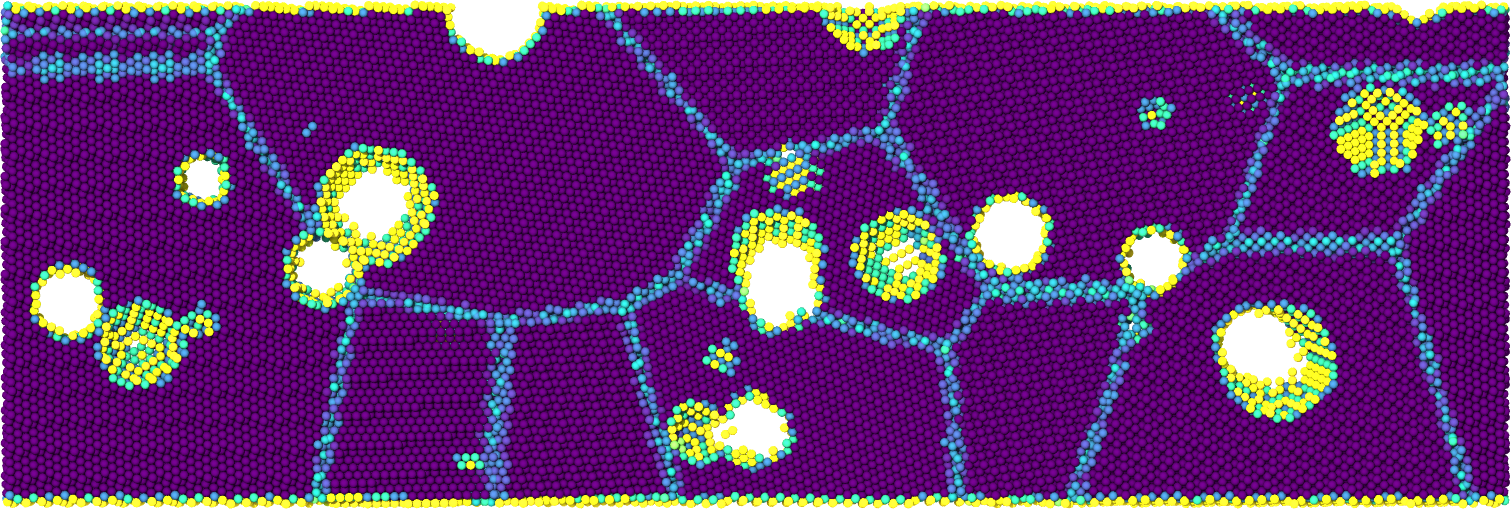
\includegraphics[width=0.85\textwidth]{fig/img_title.png}    
  \end{figure}  

  \centering \Large \textbf{Contributors:}

  \begin{center}
    \normalsize
    T. Carrard, L. Colombet, G. Chivot, O. Durand, C. Lemarchand, P. Lafourcade, J.-B. Maillet, N. Pineau, R. Prat, L. Soulard \\ \textit{add contributors}
  \end{center}

  \vfill

  \centering \Large CEA, DAM, DIF \\
  \centering \Large F-91297 Arpajon, France  
\end{titlepage}

\newpage

\tableofcontents

\newpage

\newcommand{\currentdir}{01_introduction}
\section{Introduction}
\label{sec:introduction}

\subsection{Overview}
\label{subsec:overview}

exaStamp V2 is a complete rewrite of exaStamp V1 and is based on the previous work \cite{Soulard2008}


\subsection{Features}
\label{subsec:features}



\renewcommand{\currentdir}{02_git}
\section{Using git}
\label{sec:install}

\begin{verbatim}

Setup

Prerequisites
install necessary packages as in scripts/required-packages-Ubuntu-18.04.sh

1. clone your own git repository
git clone ssh://your-inti-login@inti.ocre.cea.fr:/ccc/home/cont001/xstampdev/xstampdev/ExaStamp.git exaStamp

2. première configuration et compilation
<path-to-sources>/scripts/configure-Ubuntu-18.04.sh


How to add a remote connection to inti if you cloned from another location

3. 
git remote add inti ssh://votre-login-inti@inti.ocre.cea.fr:/ccc/home/cont001/xstampdev/xstampdev/ExaStamp.git

3b. pour faire un push ou un pull depuis/vers un depot distant :
git push inti ma-branche # push vers inti
git pull inti ma-branche # pull depuis inti

Note:
vous aurez toujours un 'remote' nommé origin qui est l'URL que vous avez utilisez pour le clone
donc si vous voulez push/pull vers le serveur duquel vous avez cloné :
git push origin ma-branche
git pull origin ma-branche

Note 2:
pour voir a liste des depot remote
git remote -v


Handling branches
copy a remote branch to the local repo, with exactly the same state as the remote one :
git checkout -b <my_new_branch> <remote>/<branch_name>
or
git reset --hard <remote>/<branch_name>

\end{verbatim}




\renewcommand{\currentdir}{03_operators}
\section{Understanding operators and YAML description}
\label{sec:operators}

\begin{verbatim}

YAML operator rules:
	- a map associated with an operator is interpredted like this: ...
	- a non map value associated with an operator is interpreted as the value of it's first declared slot

\end{verbatim}




\renewcommand{\currentdir}{04_coding_standards}
\section{Coding standards}
\label{sec:coding_stabdards}


inspired from the follwing sources
https://isocpp.org/wiki/faq/coding-standards
http://isocpp.github.io/CppCoreGuidelines/CppCoreGuidelines

\begin{lstlisting}


Coding style :
==============

class MyFirstClass
{
  // 2 spaces indent. spaces only indentation (no \t characters)
  public:
    int integer_value() const;
    void set_integer_value(int x);

  private:
    // members start with m_
    int m_integer_value;
};

class MySecondClass
{
  // 2 spaces indent. spaces only indentation (no \t characters)
  public:
    const MyFirstClass& object() const;
    void set_object(const MyFirstClass& o);

  private:
    MyFirstClass m_object;
    // class member start with s_
    static int s_per_class_integer;
};

// global values start with g_
int g_my_global_value = 0;

// function names (and member methods) use lower case only, letters and _ i.e. [a-Z0-9_] pattern
int my_function( int x, int y)
{
  // all variables are initialized
  int z = 0;
  int w = 0;
  z = x*y;
  w = x+y;
  return z/w;
}

// enum types are named (no anonymous enums)
enum Choice
{
  CHOICE_THIS,
  CHOICE_THAT,
  CHOICE_OTHER
};


// =================== Application =========================

// 1. operators in exaStampV2
// ---------------------------

// source file name is operator given name with .cpp,
// following exemple of operator named wall in exaStampV2,
// in src/compute/wall.cpp

#include "ustamp/operator.h"
// ... all necessary includes here ...
#include <iomanip>

namespace ustamp
{

  template<
    class GridT,  // if operator takes Grid<> templated type as an argument,
                  // then anonymous type with default value must ensure that instantiation is possible only if Grid<>
		  // satisfies some requirements (i.e. presence of computation scalar fields
    class = AssertGridHasFields< GridT, field::_fx, field::_fy, field::_fz, field::_ep >    >

  // class name has no real importance, but must comply to the coding standards
  class WallOperator : public OperatorNode
  {
    // input / output slots are declared private
    // if a slot is INPUT only, it must be declared either REQUIRED, OPTIONAL, or given a default value
    ADD_SLOT( GridT  , grid   , INPUT_OUTPUT );
    ADD_SLOT( Vec3d  , normal , INPUT , Vec3d{1.0,0.0,0.0} );
    ADD_SLOT( double , offset , INPUT , 0.0 );
    ADD_SLOT( double , cutoff , INPUT , REQUIRED );
    ADD_SLOT( Domain , domain , INPUT , REQUIRED );
    ADD_SLOT( double , force_scale , INPUT , OPTIONAL );

  public:

    // execute method is the only one mandatory to implement an OperatorNode
    inline void execute () override final
    {
      double fscale = 1.0;
      if( force_scale.has_value() ) // one can test if slot has a value (yaml provided or connected from an other component)
      {
	fscale = *force_scale;
      }
      // slot's value is accessed as if it would be a pointer to the value, with * or -> dereferencing
      apply_wall( *grid, *normal, - (*offset), *cutoff, *force_scale, domain->xform() );
    }

    // optional overloading to customize yaml file interpretation when describing this operator
    inline void yaml_intialize(const YAML::Node& node) override final
    {
      YAML::Node tmp;
      if( node.IsSequence() && node.size()==3 )
      {
        tmp["normal"] = node;
      }
      else { tmp = node; }
      this->OperatorNode::yaml_intialize( tmp );
    }

    // documentation method
    
  };
  
  // this helps older versions of gcc handle the unnamed default second template parameter
  template <class GridT> using WallOperatorTemplate = WallOperator<GridT>;

  // this special construction function will be automatically executed upon plugin load
  // this is useful to register this operator's factory
  CONSTRUCTOR_FUNCTION
  {
    OperatorNodeFactory::instance()->register_factory( "wall", make_grid_variant_operator< WallOperatorTemplate > );
  }

}

\end{lstlisting}



\renewcommand{\currentdir}{05_grid_cell_values}
\section{Coding standards}
\label{sec:coding_stabdards}


This describes how scalar and vector fields laying on a rectilinear grid are stored in ExaStamp.

\begin{figure}[!h]
  \centering
  \includegraphics[width=1.\textwidth]{fig/grid_cell_values.pdf} \\
\end{figure}



\bibliographystyle{unsrt}
\bibliography{biblio/biblio.bib}

\end{document}
